\textbf{\underline{OZ 9 - Wisselstroomkringen - Oefening 4:}}
\vspace{0.5cm}

In de schakeling in onderstaande figuur, neem aan dat alle parameters behalve C gegeven zijn.

\begin{enumerate}[(a)]
    \item Bepaal de stromen in functie van de tijd indien beide schakelaars gesloten zijn.
    \item Vind het vermogen geleverd aan de schakeling. \vspace{0.3cm} \\ 
\begin{minipage}{.56\textwidth}
    \item Vind de stroom in functie van de tijd na het openen van enkel schakelaar $S_1$.   
    \item Nadat schakelaar $S_2$ ook geopend is, zijn de stroom en de spanning in fase. Vind de capaciteit $C$.
    \item Vind de impedantie van het circuit wanneer beide schakelaars geopend zijn bij deze frequentie.
    \item Vind de maximale energie opgeslagen in de condensator en de spoel tijdens de oscillaties.
    \item De frequentie van de spanningsbron wordt nu verdubbeld. Vind het faseverschil tussen de stroom en de spanning.
    \item Vind de frequentie van de bronspanning die ervoor zorgt dat de inductieve reactantie de helft is van de capacitieve reactantie.
\end{minipage}
\begin{minipage}{.4\textwidth}
   \vspace{-0.5cm}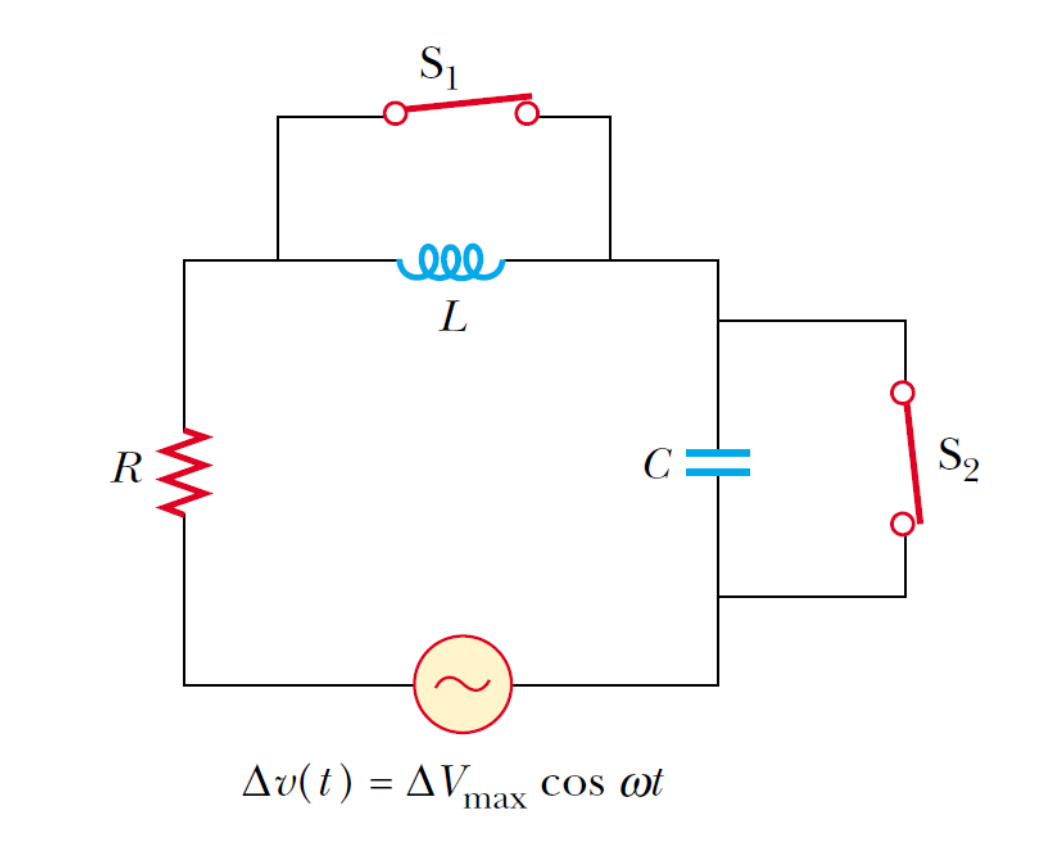
\includegraphics[scale = 0.4]{oz09/resources/Oz9Oef4.png}
\end{minipage}

\end{enumerate}

\begin{description}[labelwidth=1.5cm, leftmargin=!]
    \item[Geg. :]  $R$, $L$, $\Delta v(t) = \Delta V_\text{max} \cos(\omega t)$
\end{description}

\begin{enumerate}[(a)]
    \item 
        \begin{description}[labelwidth=1.5cm, leftmargin=!]
            \item[Geg. :]  $S_1$ en $S_2$ gesloten
            \item[Gevr. :] $i(t)$ ?
            \item[Opl. :]   
                We kunnen a\@.d\@.h\@.v\@. de weerstand een formule voor de stroom afleiden uit $v(t)$, namelijk
                \begin{equation*}
                    i(t) = \frac{\Delta v(t)}{R} = \frac{\Delta V_{\text{max}}}{R} \cos(\omega t)
                \end{equation*}
        \end{description}
    \item
        \begin{description}[labelwidth=1.5cm, leftmargin=!]
            \item[Gevr. :] $P_{\text{gem}}$ ?
            \item[Opl. :]   
                Het gemiddelde vermogen geleverd aan een wisselstroomkring, vinden we met:
                \begin{equation*}
                    P_{\text{gem}} = \frac{1}{2}I_{\text{max}}V_{\text{max}}\cos(\phi).
                \end{equation*}
                Dit kunnen we combineren met het resultaat van (a) waarbij $t = 0 \ \text{s}$ en $\phi = 0^\circ$, vinden we:
                \begin{equation*}
                    P_{\text{gem}} = \frac{1}{2}\frac{(\Delta V_{\text{max}})^2}{R}.
                \end{equation*}
        \end{description}
    \item
        \begin{description}[labelwidth=1.5cm, leftmargin=!]
            \item[Geg. :] $S_1$ open en $S_2$ gesloten
            \item[Gevr. :]  $i(t)$ ?
            \item[Opl. :]   
                We kunnen de stroom afleiden uit $\Delta v(t)$ en de impedantie van het circuit: 
                \begin{equation*}
                    i(t) = \frac{\Delta V_{\text{max}}}{Z} \cos(\omega t + \phi)
                \end{equation*}
                waarbij we moeten rekening houden met $\phi$.
        \end{description}
    \item
        \begin{description}[labelwidth=1.5cm, leftmargin=!]
            \item[Geg. :] $S_1$ open en $S_2$ open, $\phi = 0^\circ$
            \item[Gevr. :] $C$ ?
            \item[Opl. :]   
                Sinds er gegeven is dat de spanning en stroom in fase zijn en dus $\phi = 0$, volgt dat we mogen spreken van resonantie. Er volgt dus uit de resonantiehoeksnelheid:
                \begin{equation*}
                    \omega_0 = \sqrt{\frac{1}{LC}} \ \Rightarrow \ C = \frac{1}{\omega_0^2L}
                \end{equation*}
        \end{description}
    \item
        \begin{description}[labelwidth=1.5cm, leftmargin=!]
            \item[Geg. :]  $S_1$ open en $S_2$ open, $f_0$
            \item[Gevr. :] $Z$ ?
            \item[Opl. :]  
                We spreken hier van resonantie, wat betekent dat $X_L = X_C$, en dus volgt voor de impedantie:
                \begin{equation*}
                    Z = \sqrt{R^2 + (X_L - X_C)^2} = R
                \end{equation*} 
        \end{description}
        \item
        \begin{description}[labelwidth=1.5cm, leftmargin=!]
            \item[Gevr. :] $U_{\text{max}, C}$, $U_{\text{max}, L}$
            \item[Opl. :] 
            \begin{itemize}
                \item $U_{\text{max}, C}$: \\
                    De energie opgeslagen in een condensator werd gegeven door:
                    \begin{equation*}
                        U_{C} = \frac{1}{2}C(\Delta v)^2 = \frac{1}{2}Ci^2X_C^2.
                    \end{equation*}
                    Dit is maximaal als de spanning maximaal, en dus de stroom maximaal is: 
                    \begin{equation*}
                        U_{\text{max}, C} = CI_{\text{max}}^2X_C^2 = \frac{(L\Delta V_{\text{max}})^2}{2R^2}
                    \end{equation*}
                \item $U_{\text{max}, L}$: \\
                    De energie opgeslagen in een inductor werd gegeven door:
                    \begin{equation*}
                        U_{L} = \frac{1}{2}L(I)^2.
                    \end{equation*}
                    Dit is maximaal als de stroom maximaal is:
                    \begin{equation*}
                        U_{\text{max},L} = \frac{1}{2}L(I_{\text{max}})^2 = \frac{(L\Delta V_{\text{max}})^2}{2R^2}.
                    \end{equation*}
            \end{itemize}
        \end{description}
    \item
        \begin{description}[labelwidth=1.5cm, leftmargin=!]
            \item[Geg. :]  $f' = 2f_{0} \ \Rightarrow \ \omega' = 2\omega_0$ 
            \item[Gevr. :] $\phi$ ?
            \item[Opl. :]   
                We berekenen $\phi$ met de geziene formule:
                \begin{align*}
                    \phi 
                        &= \tan^{-1}\left(\frac{X_L-X_C}{R}\right) \\
                        &= \tan^{-1}\left(\frac{\omega' L - \frac{1}{\omega' C}}{R}\right) \\
                        &= \tan^{-1}\left(\frac{2\omega_0 L - \frac{1}{2\omega_0 C}}{R}\right) \\
                        &= \tan^{-1}\left(\frac{\frac{2L}{\sqrt{LC}}L - \frac{\sqrt{LC}}{2C}}{R}\right) \\
                        &= \ldots \\
                        &= \tan^{-1}\left(\frac{3}{2}\sqrt{\frac{L}{C}}\right)
                \end{align*}
        \end{description}
    \item
        \begin{description}[labelwidth=1.5cm, leftmargin=!]
            \item[Geg. :]   $X_L = \frac{1}{2}X_C$
            \item[Gevr. :]  $f'$ ?
            \item[Opl. :]   
                Als de inductieve reactantie de helft is van de capacitieve reactantie, dan volgt: 
                \begin{equation*}
                    \omega = \frac{1}{2\sqrt{LC}} = \frac{\omega_0}{2}
                \end{equation*}
        \end{description}
\end{enumerate}

% \begin{description}[labelwidth=1.5cm, leftmargin=!]
%     \item[Geg. :]   
%     \item[Gevr. :] 
%     \item[Opl. :]   
% \end{description}

\vspace{1cm}